\documentclass{article}
\bibliographystyle{plain}
\linespread{1.2}
\usepackage[margin = 1.25 in]{geometry}
\usepackage{wrapfig}
\usepackage{amsfonts}
\usepackage[utf8]{inputenc}
\usepackage[T1]{fontenc}
\usepackage{graphicx}
\usepackage[english]{babel}
\usepackage[algoruled]{algorithm2e}

\renewcommand{\theequation}{\thesection.arabic{equation}}

\renewcommand{\thefigure}{\thesection.\arabic{figure}}



\renewcommand{\vec}[1]{\mathbf{#1}}
\renewcommand{\theequation}{\thesubsection.\arabic{equation}}
\DeclareGraphicsExtensions{.pdf,.png,.jpg, .gif}

\usepackage{amsthm}

\usepackage[english]{babel}
\usepackage{mathtools}

%\usepackage[OT2,T1]{fontenc}
%\DeclareSymbolFont{cyrletters}{OT2}{wncyr}{m}{n}
%\DeclareMathSymbol{\sha}{\mathalpha}{cyrletters}{"58}

\DeclareFontFamily{U}{wncy}{}
\DeclareFontShape{U}{wncy}{m}{n}{<->wncyr10}{}
\DeclareSymbolFont{mcy}{U}{wncy}{m}{n}
\DeclareMathSymbol{\Sh}{\mathord}{mcy}{"58} 
\DeclareMathOperator*{\argmin}{arg\,min}

\newcounter{eqn}
\renewcommand*{\theeqn}{\alph{eqn})}
\newcommand{\num}{\refstepcounter{eqn}\text{\theeqn}\;}

\makeatother
\newcommand{\vectornorm}[1]{\left|\left|#1\right|\right|}
\newcommand*\conjugate[1]{\bar{#1}}

\newtheorem{thm}{Theorem}
\newtheorem{defn}{Definition}
 %\theoremstyle{plain}
  \newtheorem{theorem}{Theorem}[section]
  \newtheorem{corollary}[theorem]{Corollary}
  \newtheorem{proposition}[theorem]{Proposition}
  \newtheorem{lemma}[theorem]{Lemma}
\newtheorem{example}[theorem]{Example}
  \newtheorem{definition}[theorem]{Definition}
  \newtheorem{conj}[theorem]{Conjecture}
 \newtheorem{condition}{Condition}
 \newtheorem{remark}[theorem]{Remark}

\newcommand{\supp}{\operatorname{supp}} 
\newcommand{\vc}[1]{{\mathbf{ #1}}}
\newcommand{\tn}{\widetilde{\nabla}_{n} }
\newcommand{\Z}{{\mathbb{Z}}}
\newcommand{\re}{{\mathbb{R}}}
\newcommand{\II}{{\mathbb{I}}}
\newcommand{\ep}{{\mathbb{E}}}
\newcommand{\pr}{{\mathbb{P}}}
\newcommand{\FF}{{\mathcal{F}}}
\newcommand{\TT}{{\mathcal{T}}}
\newcommand{\phin}{\phig{n}}
\newcommand{\phig}[1]{\phi^{(#1)}}
\newcommand{\ol}[1]{\overline{#1}}
\newcommand{\eff}{{\rm eff}}
\newcommand{\suc}{{\rm suc}}
\newcommand{\tends}{\rightarrow \infty}
\newcommand{\setS}{{\mathcal{S}}}
\newcommand{\setP}{{\mathcal{P}}}
\newcommand{\setX}{{\mathcal{X}}}
\newcommand{\nec}{{\rm nec}}
\newcommand{\bd}{{\rm bd}}

\DeclareUnicodeCharacter{00A0}{~}

\title{Compressive Filtering}
\author{Tom Kealy}

\begin{document}
\maketitle

\section{Classical Filtering and Compressive Sensing}

Compressive Sensing has established that non-uniform sampling with random waveforms can be used to capture low-complexity signals, at rates far below those specified by Nyquist. The work of Candes and Tao \cite{Candes2006} and Donoho \cite{donoho2006compressed} has established that this sensing framework is universal: the sensing mechanism and reconstruction algorithms are insensitive as to whether the signal is an image, a song, or frequency spectra as long as it is sparse. The computational effort in these systems is backloaded to the reconstruction algorithm, which can have considerable computational complexity. This is in contrast to traditional sampling \cite{unser}, where the processing required to obtain the digital samples is the difficult part. Classical reconstruction is simply interpolation through an appropriate filter.

There are some technical specifications that on the compressive sensing mechanism which means that it can achieve this dimensionality reduction. Firstly the sensing waveforms must be incoherent with the signals being sensed \cite{candes2008introduction}. This is a statement similar to the \(T_s\)-spaced delta function requirement from classical sensing: we need to sample the signal in a domain where its information is spread out. As a signal cannot be sparse in two bases simultaneously, we can exploit the uncertainty relation between the bases to sample the signal efficiently. The other requirement on the sensing waveforms is that they are orthogonal, and change the norm of the signal by very little. In particular, they must not send the signal to \(0\), or recovery would be impossible.

The structure of this document is as follows: sections \eqref{sec:prelims}, is a literature review of relevant material from compressed sensing, Wishart matrices, and maximum likelihood estimation of uncompressed signals in noise. Section \eqref{sec:estimation} gives an overview of the problem of estimating a signal from a known set of basis functions. 

\subsection{Classical Sampling}

Classically, for perfect signal reconstruction, we must sample a signal such that the sampling rate must be at least twice the maximum frequency in the bandlimited signal \cite{unser}. The continuous time signal can then be recovered using an appropriate reconstruction filter (e.g. a sinc filter). For example, we can represent a sampled continuous signal as a multiplication of the signal with a train of Dirac delta functions at multiples of the sampling period T.
%
\begin{equation}
x\left(nT\right) = \Sh\left(t-nT\right)x\left(t\right)
\end{equation}
%
where
%
\begin{equation}
\Sh\left(t-nT\right) = \sum_{k=-\infty}^{\infty} \delta\left(t - kT\right)
\end{equation}

Working the frequency domain, this multiplication becomes convolution (which is equivalent to shifting):

\begin{equation}
\hat{X}_{s}\left(f\right) = \sum_{k=-\infty}^\infty x\left(t - kT\right)
\end{equation}

Thus if the spectrum of the frequency is supported on the interval \(\left(-B, B\right)\) then sampling at intervals \(\frac{1}{2B}\) will contain enough information to reconstruct the signal \(x(\left(t\right)\). Multiplying the spectrum by a rectangle function (low-pass filtering), to remove any images caused by the periodicity of the function, and the signal \(x(\left(t\right)\) can be reconstructed from its samples:

\begin{equation}
x\left(t\right) = \sum_{n=-\infty}^\infty x\left(nT\right) sinc\left(\frac{t_nT}{T}\right)
\end{equation}


\subsection{Maximum Likelihood estimation: non-compressive case}\label{sec:max-like}

Consider a received signal \(y \in \re^n\), composed of a deterministic signal \(\bar{s} \in \re^n\) corrupted by noise \(n \in \re^n\) (assumed to have zero mean and unit variance), i.e.

\begin{equation}
y = s + n
\end{equation}

We assume \(s\left(\Theta\right)\) comes from a fixed class of signals, with parameters indexed by a set \(\Theta\). For example

\begin{itemize}
\item The signal \(s\) is composed of a single frequency with unit amplitude \(s = e^{i \omega_0 k}\). In this case \( \Theta = \{\omega_j\}_{j=1}^n \) is the set of possible frequencies the signal may take on.

\item The signal \(s\) is a scaled and shifted version of a model signal \(f\): \(s(t) = Cf\left(t - \tau\right)\). In this case \(\Theta = \left(C, \tau \right)\).

\item The signal \(s\) can be expanded in some orthonormal basis, and that we have access to the basis functions \(\{\phi_i\}_{i=1}^n\):
\begin{equation}
s = \sum_{i=1}^n \alpha_i \phi_i
\end{equation}

In this case \(\Theta = \{\alpha_i, \phi_i\}_{i=1}^n\)

\end{itemize}

We can write the likelihood for \(y\) down as, for a given \(\Theta\), \(s\) is deterministic. Therefore y is a Gaussian random variable with mean \(s\):

\begin{equation}
f\left(y \mid s\right) = \left(\frac{1}{\sqrt{2\pi}} \right)^n \exp{\left( - \frac{\left(y-s(\Theta)\right)^T\left(y-s(\Theta)\right)}{2} \right)}
\end{equation}

Maximising this is equivalent to maximising:

\begin{equation}
\ln f\left(\Theta\right) = -\vectornorm{y}_2^2 + 2\langle y, s\left(\Theta\right)\rangle - \vectornorm{s}_2^2
\end{equation}

Since the terms \(\vectornorm{y}_2^2\) and \(\vectornorm{s}_2^2\) do not change, we can write the ML estimate of \(\Theta\) as:

\begin{equation}
\hat{\Theta} = \argmax_{\Theta} \langle y, s\left(\Theta\right)\rangle
\end{equation}

So, for example:

\begin{itemize}
\item If we receive a single tone corrupted by noise \(y = e^{i \omega_0 k} + n\) then we can estimate \(\omega_0\) by calculating \(\argmax_{\omega_i} \langle y, e^{i \omega_j k}\rangle = e^{i \omega_0 k}\) as the functions \(e^{i \omega_0 j k }\) are orthonormal: \(\langle e^{i \omega_l k}, e^{i \omega_r k} \rangle = \delta_{lr}\).

\item If we receive a signal composed of a sum of orthonormal basis functions we can estimate the coefficients \(\alpha_i\) as:

\begin{align}
\langle y, \phi_i\rangle\ =& \sum_{j=1}^n \alpha_j \phi_j^T\phi_i + n^T\phi_i \\
=& \alpha_i + \varepsilon_i
\end{align}

where \(\varepsilon_i = \langle n^T, \phi_i \rangle \) is some small error. Thus the maximum likelihood estimate of \(s\) is:

\begin{equation}
\hat{s} = \sum_{i=1}^n \hat{\alpha}_i \phi_i
\end{equation}

where

\begin{equation}
\hat{\alpha} = \langle y, \phi_i \rangle
\end{equation}

\end{itemize}

\subsection{Compressive Sensing Preliminaries} \label{sec:prelims}

In contrast to Classical Sensing, Compressive Sampling suggests that by adding randomness into the measurement process, a sparse (or compressible signal) may be accurately sensed with far fewer measurements:

Given a signal \(x \in \re^n\), a matrix \(A \in \re^{m \times n}\) we can acquire the signal via the set of linear measurements:

\begin{equation}
y = Ax
\end{equation}

where in this case \(A\) represents the sampling system. In contrast to classical sensing, which requires that \(m = n\) for there to be no loss of information, it is possible to reconstruct \(x\) from an under-determined set of measurements as long as \(x\) is sparse in some basis. 

To make this precise, we define \(\Sigma_s\) as the set of \(s\)-sparse signals in \(\re^n\):

\begin{definition}
\begin{equation}
\Sigma_s = \{ x \in \re^n : \mathrm{supp}\left(x\right) \leq s\}
\end{equation}
where \(\mathrm{supp}\left(x\right) \) is the set of indices on which \(x\) is non-zero.
\end{definition}

Some technical conditions on the matrix \(A\) have to satisfied for it: namely the transformation defined by \(A\) must behave like an approximate Isometry, and it must be incoherent.

\begin{definition}[RIP]
We say that a matrix \(A\) satisifes the RIP of order \(s\) if there exists a \(\delta \in \left(0, 1\right)\) such that for all \(x \in \Sigma_s\):

\begin{equation}
\left(1 - \delta\right) \vectornorm{x}_2^2 \leq \vectornorm{Ax}_2^2 \leq \left(1 + \delta\right) \vectornorm{x}_2^2
\end{equation}
i.e. \(A\) approximately preserves the lengths of all \(s\)-sparse vectors in \(\re^n\). 
\label{def:RIP}
\end{definition}

\begin{definition}[Coherence]
The mutual coherence of a matrix \(A\) is the absolute normalised inner product between different columns from \(A\). Denoting the \(k\)-th column in \(A\) by \(a_k\), the mutual coherence is given by:
\begin{equation}
\mu(A) = \max_{1\leq i,j\leq n , i\neq j} \frac{|\langle a^T_i, a_j\rangle|}{\vectornorm{a_i}_2\vectornorm{a_j}_2}
\end{equation}
\end{definition}

This implies that sensing with incoherent systems is good, and efficient mechanisms ought to acquire correlations with random waveforms (e.g. white noise).

\begin{remark} [Information Preservation]
A necessary condition to recover all \(s\)-sparse vectors from the measurements \(Ax\) is that \(Ax_1 \neq Ax_2\) for any pair \( x_ \neq x_2\), \(x_1, x_2 \in \Sigma_s\), which is equivalent to \(\vectornorm{A\left(x_1 - x_2\right)}_2^2 > 0\). 

This is guaranteed as long as \(A\) satisfies the RIP of order 2\(s\) with constant \(\delta\) - as the vector \(x_1 - x_2\) will hve at most \(2s\) non-zero entries, and so will be distinguishable after multiplication with \(A\). To complete the argument take \(x = x_1 - x_2\) in definition \eqref{def:RIP}, guaranteeing \(\vectornorm{A\left(x_1 - x_2\right)}_2^2 > 0 \), and requiring the RIP order of \(A\) to be \(2s\).
\end{remark}

\begin{remark} [Stability]
We also require that the dimensionality reduction of compressed sensing is the preservation of relative distances: that is if \(x_1\) and \(x_2\) are far apart in \(\re^n\) then their projections \(Ax_1\) and \(Ax_2\) are far apart in \(\re^m\). This will guarantee that the dimensionality reduction is robust to noise. 
\end{remark}

A requirement on the matrix \(A\) that satisfies both of these conditions is the following:

\begin{definition}[\(\delta\)-stable embedding]
We say that a mapping is a \(\delta\)-stable embedding of \(U,V \subset \re^n\) if

\begin{equation}
\left(1 - \delta \right) \vectornorm{u-v}_2^2 \leq \vectornorm{Au-Av}_2^2 \leq \left(1 + \delta\right) \vectornorm{u-v}_2^2
\end{equation}

for all \(u \in U\) and \(v \in V\). 
\label{def:d-stable}
\end{definition} 

\begin{remark}
Note that a matrix \(A\), satisfying the RIP of order \(2s\) is a \(\delta\)-stable embedding of \(\Sigma_s, \Sigma_s\). 
\end{remark}

\begin{remark}
Definition \ref{def:d-stable} has a simple interpretation: the matrix \(A\) must approximately preserve Euclidean distances between all points in the signal model \(\Sigma_s\).
\end{remark}



\textbf{Theorem} \cite{Candes2006}
Fix x \(\in \mathbb{R}^n\) with a sparse coefficient basis, \(x_{i}\) in \(\psi\). Then a reconstruction from \(m\) random measurements is possible with probability \(1 - \delta\) if: 

\begin{equation}
m \geq C \mu^2(A) S \log\left(\frac{n}{\delta}\right)
\end{equation}
\label{minsamples}

where \( \mu(A)\) is the coherence of the two bases, and \(S\) is the number of non-zero entries on the support of the signal. 

In this new sensing paradigm, the complexity is shifted to the reconstruction process, where with high probability Donoho proved \cite{donoho2004neighborly}, that the minimiser of the program:

\begin{equation}
\argmin_{x} \frac{1}{2}\vectornorm{y-Ax}_2^2 + \lambda\vectornorm{x}_1
\end{equation}

coincides with the sparsest solution to the under-determined system of linear equations. Thus we are able to sense sparse signals with random waveforms, and reconstruct them via linear programming.

Reconstruction isn't the only signal processing task: it is often part of a chain of operations. For example, we may require high frequency components of the received signal to be filtered out, or for timing and phase synchronisation in demodulation. Using Compressive sensing in these chains is less attractive: current methodology is to reconstruct the signal and then process the Nyquist samples using traditional techniques. The processing chain is then limited by the speed of the reconstruction step. 

The foundational ideas of compressive sensing suggest, however, that reconstruction may be unnecessary. Compressive samples contain (almost) all the information about the signal, and are acquired via a linear process. This suggests that there may be some operations directly on the samples which can be used to extract information about the original signal, but which avoids costly reconstruction. I.e. for signal processing tasks where some other metric is the end result of the processing chain (e.g. classification), reconstructing Nyquist samples is optimal. This has an added benefit: it may be possible to further reduce the sampling rate, as we are no longer constrained by the requirement to reconstruct the samples.

The papers \cite{davenport2010signal} and \cite{davenport2007smashed} provide an introductory answer for the cases of filtering, detection, classification and estimation.


\subsection{Random Matrix Constructions} \label{sec:mtx-contruction}

To construct matrices satisfying definition \ref{def:d-stable}, given \(m, n\) we generate \(A\) by \(A_{ij}\) being i.i.d random variables from distributions with the following conditions \cite{davenport2010signal}

\begin{condition}[Norm preservation]
\(\ep A_{ij}^2 = \frac{1}{m}\)
\label{cond:norm-pres}
\end{condition}

\begin{condition}[sub-Gaussian]
\(\ep\left( e^{A_{ij}t} \right) \leq e^{C^2 t^2 /2}\)
\label{cond:sub-Gauss}
\end{condition}

\begin{lemma}[Concentration]
There exists constants, for all t, such that random variables \(A_{ij}\) satisfying conditions \eqref{cond:norm-pres} and \eqref{cond:sub-Gauss} satisfy the following concentration inequality \cite{baraniuk2008simple}, \cite{Devore09instanceoptimalityin}[Lemma 6.1]:

\begin{equation}
\pr\left( \biggl\lvert \vectornorm{Ax}_2^2 - \vectornorm{x}_2^2 \biggr\rvert \geq \varepsilon  \vectornorm{x}_2^2 \right) \leq 2e^{-cM\varepsilon^2}
\label{cond:sub-Gauss concetration}
\end{equation} 
\end{lemma}

Then in \cite{baraniuk2008simple} the following theorem is proved:

\begin{theorem}
Suppose that \(m\), \(n\) and \(0 < \delta < 1\) are given. If the probability distribution generating \(A\) satisfies condition \eqref{cond:sub-Gauss concetration}, then there exist constants \(c_1, c_2\) depending only on \(\delta\) such that the RIP \eqref{def:RIP} holds for \(A\) with the prescribed \(\delta\) and any  \(s \leq \frac{c_1 n}{\log{n/s}}\) with probability \(\geq 1-2e^{-c_2n}\) 
\end{theorem}

For example, if we take \(A_{ij} \sim \mathcal{N}\left(0, 1/m\right)\), then the matrix \(A\) will satisfy the RIP 

\subsection{Wishart Matrices}

Let \(X\}\) be a an \(n \times p\) random matrix, each row of which is drawn from the \(p\)-variate normal distribution with mean 0 and covariance matrix \(H\).

\begin{equation}
X_i = \left(x_1^{(i)}, \ldots , x_p^{(i)}\right) \sim N\left(0, H\right)
\end{equation}


\begin{definition}[Wishart Matrix \cite{eaton2007wishart}]
Let 

\begin{equation}
W_n = X^T X
\end{equation}

Then \(W \in \re^{p \times p}\) has the Wishart distribution with parameters 

\begin{equation}
W_p\left(H, n\right)
\end{equation}

where \(p\) is the number of degrees of freedom.
\end{definition}

\begin{remark}
This distribution is a generalisation of the Chi-squared distribution: let \(p = H = 1\). 
\end{remark}

\begin{theorem}[Expected Value]
\begin{equation}
\ep\left(W\right) = rH
\end{equation}
\end{theorem}
\begin{proof}
\begin{align*}
\ep\left(W\right) &= \ep\left(\sum_{j=1}^r X_j X_j^T\right) \\
&= \sum_{j=1}^r \ep\left(X_jX_j^T\right) \\
&= \sum_{j=1}^r \left( \mathrm{Var}(X_j) + \ep(X_j) \ep(X_j^T)   \right) \\
&= rH 
\end{align*}
Where the last line follows as \(X_j\) is drawn from a distribution with zero mean.
\end{proof}

\begin{remark}
The matrix \(M = A^TA\), where \(A\) is constructed by the methods from section \ref{sec:mtx-contruction}, will have a Wishart distribution. In particular, it will have \(\ep M = \frac{1}{m}I_n\) 
\label{remark: exp AtA}
\end{remark}

The joint distribution of the eigenvalues is given by \cite{levequeMatrices}:

\begin{equation}
p\left(\lambda_1, \ldots, \lambda_r\right) = c_r \prod_{i=1}^r e^{-\lambda_i}\prod_{i<j}\left(\lambda_i - \lambda_j\right)^2
\end{equation}

The eigenvectors are uniform on the unit sphere in \(\re^{r}\).

\section{Compressive Estimation} \label{sec:estimation}
In this section, we develop some intuition into constructing estimators for the signal \(s\) directly on the compressive measurements:

\begin{theorem}

Given a set of measurements of the form:

\begin{equation}
y = As + n
\end{equation}
\\
where \(A \in \re^{m \times n} \), \(A_{ij} \sim \mathcal{N}\left(0,1/m\right)\), and \(n \in \re^n\) is AWGN i.e. \(\sim N\left(0, \sigma^2 I\right)\). We again assume that \(s\) comes from a fixed set of models, parametrised by some set \(\Theta\). 

Then, the maximum likelihood estimator of \(s\), for the case where \(s\) can be expanded in an orthonormal basis \(s = \sum_{i=1}^n \alpha_i\phi_i\):

\begin{equation}
\hat{s} = \sum_{i=1}^n m\langle y, A\phi_i\rangle \phi_i
\end{equation}

\end{theorem}
\begin{proof}
The likelihood for this model is, (as y is a normal random variable):

\begin{equation}
f\left(y \mid s\right) = \left(\frac{1}{\left(2\pi\right)^{n/2}} \right)\exp{\left( - \frac{\left(y-As\right)^T  \left(y-As\right)}{2} \right)}
\end{equation}

Taking the logarithm and expanding, we find

\begin{equation}
\ln{f\left(y \mid s\right)} = -y^Ty - s^TA^TAs + 2\langle y, As \rangle + c
\end{equation}

which is equal to:

\begin{equation}
ln{f} = - \vectornorm{y}_2^2 - \vectornorm{As}_2^2 + 2\langle y, As \rangle
\label{log-like}
\end{equation}

(where the constant has been dropped). The first term of \eqref{log-like} is constant, for the same reasons as in section \eqref{sec:estimation}. The term 

\begin{equation}
\vectornorm{As}^2_2 = \langle As, As\rangle
\end{equation}

can be written as 

\begin{equation}
\langle A^T As, s\rangle
\label{ata}
\end{equation}

We will assume that \(A^TA\) concentrates in the sense of \ref{cond:sub-Gauss concetration} and replace \ref{ata} with its expectation \(\ep{\left( \langle A^T As, s\rangle \right)}\)

\begin{align*}
\ep{\left(\langle A^T As, s\rangle\right)} &=  \ep{\sum_{i=1}^n (A^TAs)^T_i s_i} \\
&= \sum_{i=1}^n \ep{(A^TAs)_i s_i} \\
&= \sum_{i=1}^n (\frac{1}{m}e_i s_i)^T_i s_i \\
&= \frac{1}{m} \langle s, s \rangle
\end{align*}

because

\begin{equation}
\ep{A^TA} = \frac{1}{m}I
\end{equation}

as it is a Wishart matrix (see section\ref{sec:prelims}). 
\\
So we can further approximate \eqref{log-like}:

\begin{equation}
\ln{f\left(y \mid s\right)}  = - \vectornorm{y}_2^2 - \frac{1}{m}\vectornorm{s}_2^2 + 2\langle y, As \rangle
\label{approx-log-like}
\end{equation}

The only, non-constant part of \eqref{approx-log-like} is the third term and so we define the estimator:

\begin{equation}
\hat{s} = \argmax_{\Theta} \langle y , As\left(\Theta\right)\rangle
\label{eq: compressive-estimator}
\end{equation}
\end{proof}

\begin{corollary}
Consider the case where \( y = As\) (no noise). Then

\begin{align*}
y^TA\phi_j &= \sum_i \alpha_i \phi_i^TA^TA\phi_j
\end{align*}



So 


\begin{align*}
y^TA\phi_j &= \sum_i \alpha_i \phi_i^TA^TA\phi_j \sim \frac{\alpha_i}{m} \delta_{ij}
\end{align*}

giving
 
\begin{equation}
\widehat{\alpha_i} = m\left(y^TA\phi_j\right)
\end{equation}
\end{corollary}

\begin{remark}
The matrix \(M = A^TA\) is the projection onto the row-space of \(A\). It follows that \(\vectornorm{Ms}_2^2\) is simply the norm of the component of \(s\) which lies in the row-space of \(A\). This quantity is at most \(\vectornorm{s}_2^2\), but can also be \(0\) if \(s\) lies in the null space of \(A\). However, because \(A\) is random, we can expect that \(\vectornorm{Ms}_2^2\) will concentrate around \(\sqrt{m/n}\vectornorm{s}_2^2\) (this follows from the concentration property of sub-Gaussian random variables \eqref{cond:sub-Gauss concetration}).
\end{remark}

\begin{example}{Example: Single Spike}
We illustrate these ideas with a simple example: estimate which of \(n\) frequencies \(s\) is composed of.

A signal \(s \in \re^{300}\) composed of a single (random) delta function, with coefficients drawn from a Normal distribution (with mean 100, and variance 1) i.e 

\begin{equation}
s = \alpha_i \delta_i
\end{equation}
\\
with 

\begin{equation}
a_i \sim \mathcal{N}\left(100, 1\right)
\end{equation}

and the index \(i\) chosen uniformly at random from \([1, n]\).
\\
The signal was measured via a random Gaussian matrix \(A \in \re^{100 \times 300}\), with variance \(\sigma^2 = 1/
100 \) and the inner product between \(y = As\) and all 300 delta functions projected onto \(\re^{100}\) was calculated:

\begin{equation}
\hat{\alpha}_j = m\langle (A\alpha_i\delta_i), A\delta_j \rangle
\end{equation} 

We plot the \(\hat{\alpha_j}\) below, figure \ref{fig:new_basis_25}, (red circles), with the original signal (in blue, continuous line). Note how the maximum of the \(\hat{\alpha_j}\), coincides with the true signal.

\begin{figure}[h]
\centering
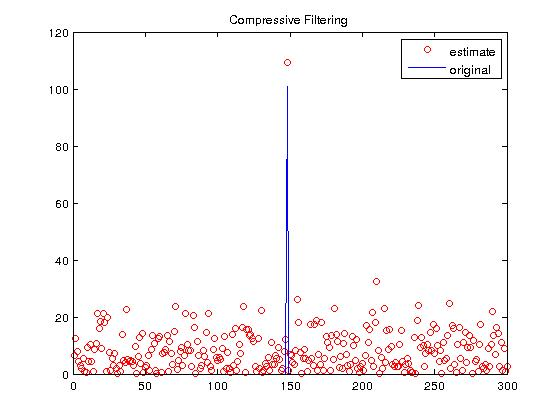
\includegraphics[height = 7.3 cm]{1spike_legend.jpg}
\caption{}
\label{fig:new_basis_25}
\end{figure}
\end{example}
\section{Estimating Frequency Spectra}\label{sec:freq-model}

\subsection{Estimating a single rectangle}

We show how to estimate a signal, composed of a single rectangle \eqref{fig:rectangle} expanded in the following basis

\begin{equation}
l_i\left(x\right) =
\begin{cases}
1 & \text{if } x \leq i \\
0 & \text{ otherwise } 
\end{cases}
\label{basis}
\end{equation}

That is, \(l_i\) is a left-hand step function. 

The basis (\ref{basis}) can be expressed as a matrix in \(\re^{n \times n}\) as:

\begin{equation}
L = \begin{pmatrix}
 1 & 0 & 0 & 0  & 0 \ldots 0 \\
  1 & 1 & 0 & 0  & 0 \ldots 0\\
     1 & 1 & 1 & 0  & 0 \ldots0  \\
    \ldots  \\
     1 & 1 & 1 & 1  & 1 \ldots 1 
\end{pmatrix}
\label{lower-L}
\end{equation}

By direct computation, this inverse of \(L\) is:

\begin{equation}
D = \begin{pmatrix}
 1 & 0 & 0 & 0  & 0 \ldots 0 \\
  -1 & 1 & 0 & 0  & 0 \ldots 0\\
     0 & -1 & 0 & 0  & 0 \ldots0  \\
    \ldots  \\
     0 & 0 & 0 & 0  \ldots -1 & 1
\end{pmatrix}
\label{inv-L}
\end{equation}

We model our PSD signal \(g\) as a linear combination of the basis functions (\ref{basis}):

\begin{equation}
g\left(x\right) = \sum_i a_i l_i\left(x\right) = L^Ta
\label{basis-expansion}
\end{equation}

where \(a = (a_1, \ldots, a_n\) are the coefficients in this basis expansion, and \(l_i\) are the rows of \(L\). Note that as defined, \(g\) is a column vector.

\begin{proposition}
\begin{equation}
D^Tg = a
\end{equation}
\label{def:a}
\end{proposition}
\begin{proof}

\begin{align}
D^Tg &= D^T L^T a \\
&= \left(LD\right)^Ta \\
&= a
\end{align}

as \(LD = I\).

\end{proof}

We define the inner product between two vectors as follows:

\begin{definition}
\begin{equation}
\langle x, y \rangle = x^T y = \sum_i x_i y_i
\end{equation}	
where \(x_i, y_i\) are the components of the vectors \(x,y\) in the \(i^{th}\) direction with respect to some basis vectors \(e_i\).
\end{definition}

We can define a matrix representation for the set of basis vectors \(l_i\), by taking all inner products between all pairs basis vectors:

\begin{definition}
\begin{equation}
F_{n, ij} = \langle l_i, l_j \rangle
\end{equation}

This matrix has the representation:

\begin{equation}
F_{ij} = min(i,j)
\end{equation}

An example of such a matrix is:

\begin{equation}
F_n= \begin{pmatrix}
 1 & 1 & 1 & 1  & 1 \\
  1 & 2 & 2 & 2  & 2\\
     1 & 2 & 3 & 3  & 3  \\
    1 & 2 & 3 & 4  & 4  \\
     1 & 2 & 3 & 4  & 5 
\end{pmatrix}
\label{def:Fmtx}
\end{equation}
\end{definition}

This matrix is invertible.

\begin{theorem}
\begin{equation}
det(F_n) = 1
\end{equation}
\end{theorem}
\begin{proof}
Consider the matrix \(F_n\). Subtract the \(n-1\)th column from the \(n\)th. We obtain a matrix with \(0\) on the final column except the entry \(F_n(n,n) = 1\). Since the top \((n-1) \times (n-1)\) is \(F_{n-1}\) we find that 

\begin{equation}
det(F_n) = 1 \times det(F_{n-1})
\end{equation} 

By recursion and \(det(F_1) = 1\) we have \(det(F_n) = 1\).

\end{proof}

This matrix can be factorised as \(F = LL^T\).

From this it follows that

\begin{equation}
F^{-1} = \begin{pmatrix}
 2 & -1 & 0 & 0  & 0 \ldots 0 \\
  -1 & 2 & -1 & 0  & 0 \ldots 0\\
     0 & -1 & 2 & -1  & 0 \ldots0  \\
    \ldots  \\
     0 & 0 & 0 & 0  \ldots -1 & 1 
\end{pmatrix}
\end{equation}

To find the \(a_i\), we correlate (take the inner product of) the signal against the basis (\ref{basis}).

\begin{definition}
\begin{align}
h_j &= \langle g, l_j \rangle \\
&= \sum_j g\left(x\right) l_j\left(x\right) \\
&= \sum_j a_i l_i\left(x\right) l_j\left(x\right) \\
&= a_i \langle l_i, l_j\rangle \\
&\left(= \sum_{x=1}^j g\left(x\right)\right)
\end{align}

In matrix language \(h = F a^T\). This is the inner product between the signal \(g\) and the basis functions \(l_i\).
\end{definition}

\begin{figure}[h]
\centering
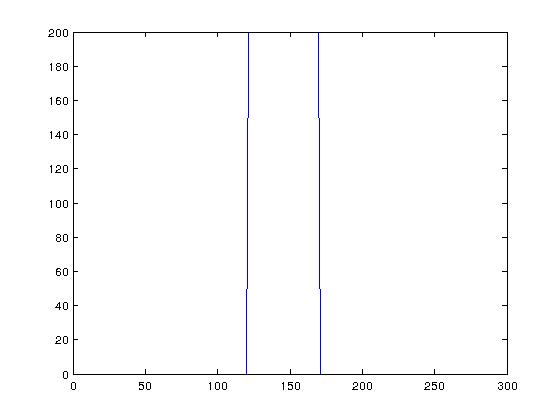
\includegraphics[height = 7.3 cm]{g.jpg}
\caption{}
\label{fig:rectangle}
\end{figure}

Given a set of compressive measurements: 

\begin{equation}
y = Ag
\end{equation}
\\
where \(A \in \re^{m \times n} \), \(A_{ij} \sim \mathcal{N}\left(0,1/m\right)\).
\\
We then compute 
\begin{equation}
\langle y, Al_i\rangle = a_j  l_j^TA^tAl_j \sim \frac{a_j}{m} \langle l_j, l_i \rangle
\end{equation}
for the set of basis vectors \(l_1 \ldots l_n\) i.e. the estimator from the previous section, corresponding to this set of basis functions \eqref{eq: compressive-estimator}. 

We then form the vector 

\begin{equation}
\hat{h} = m \sum_i \langle y, Al_i\rangle l_j \sim h
\label{ss-estimator}
\end{equation}

An example can be seen in figure \ref{fig:hhat}, for a matrix \(A \in \re^{200 \times 300}.\)

\begin{figure}[h]
\centering
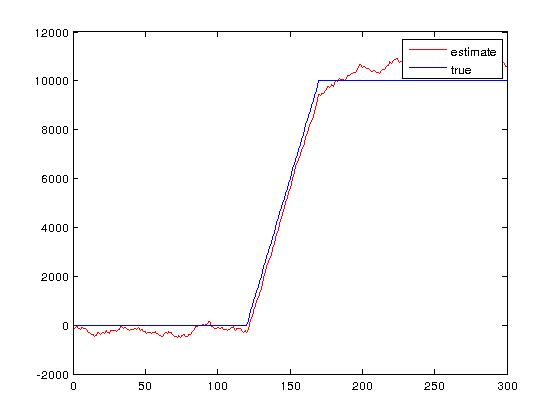
\includegraphics[height = 7.3 cm]{hhat.jpg}
\caption{}
\label{fig:hhat}
\end{figure}

\subsection{Estimating Frequency spectra}

Continuing from the previous (sub)-section we can create an estimate of \(g\), by the following procedure:

\begin{itemize}
\item Estimate the coefficients of the basis \(\hat{a}\) using \(\hat{a} = F^{-1} \hat{h}\)
\item Choose the \(k\) largest (for some \(k\) to be determined later).
\item Between the indices of the \(k\) \(\hat{a}\) take the average of the signal \(L^{-1}\hat{h}\).
\item For each piece between the \(k\) changepoints, do a t-test to determine whether the signal is noise, or a transmission.
\end{itemize}

Some examples of the output of this procedure are shown below, for synthetic and real (Ofcom) data.


\begin{figure}[h]
\centering
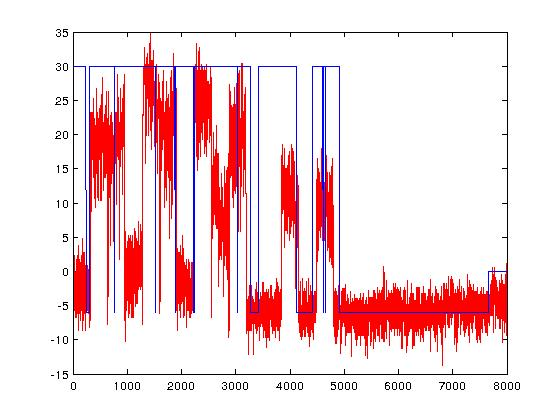
\includegraphics[height = 7.3 cm]{ofcom_classification.jpg}
\caption{}
\label{fig:hvb}
\end{figure}

\begin{figure}[h]
\centering
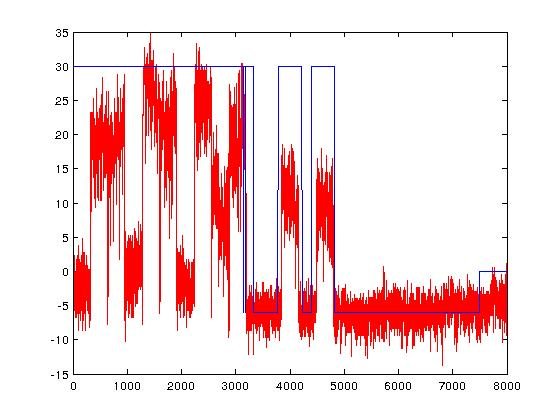
\includegraphics[height = 7.3 cm]{ofcom_classification1.jpg}
\caption{}
\label{fig:hvb}
\end{figure}

\begin{figure}[h]
\centering
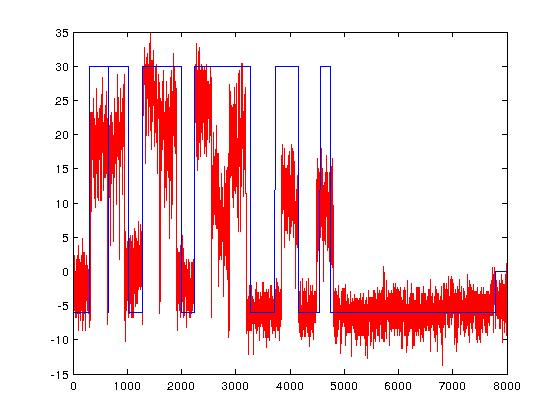
\includegraphics[height = 7.3 cm]{higher_noise_floor0.jpg}
\caption{}
\label{fig:hvb}
\end{figure}

\begin{figure}[h]
\centering
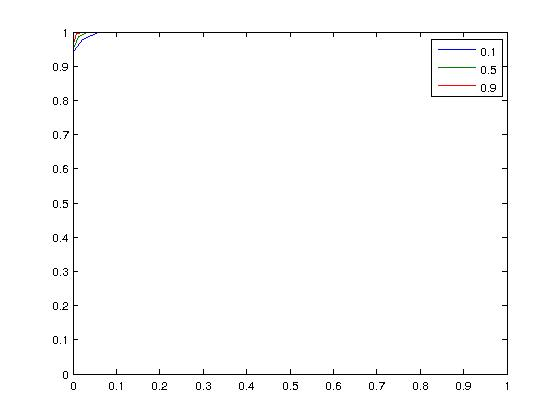
\includegraphics[height = 7.3 cm]{many_roc.jpg}
\caption{}
\label{fig:hvb}
\end{figure}

\section{Time-Frequency Model}
In this section we extend the model from section \ref{sec:freq-model}, to jointly estimate a collection of signals sensed over time. 

In this case, we have a series frequency spectra \(\in \re^n\), sensed at \(T\) time instants. We extend the model, again in the same basis:


\begin{equation}
l_{i,t}\left(x, \tau\right) = \mathbb{I}\left(t \leq \tau \right)\mathbb{I}\left(x \leq i\right)
\label{time-freq basis}
\end{equation}

We can express these basis functions in terms of the basis functions \eqref{basis}, and similarly defined basis functions over time:

\begin{equation}
l_t\left(\tau\right) =
\begin{cases}
1 & \text{if } t \leq \tau \\
0 & \text{ otherwise } 
\end{cases}
\label{time-basis}
\end{equation}

That is, \(l_t\) is again a left-hand step function. 

\begin{proposition}
\begin{equation}
l_{i,t}\left(x, \tau\right) = l_i\left(x\right) \kronecker l_t\left(\tau\right)
\end{equation}
\begin{proof}
Consider a fixed frequency, w.l.o.g \(i=1\). Then 
\begin{equation}
l_{1,t}\left(x, \tau\right) = \mathbb{I}\left(x \leq 1\right)\mathbb{I}\left(t \leq \tau \right)
\end{equation}
There are \(T\) possible vectors, each of length \(n\), for this combination of \(\left(i,t\right)\). Therefore \(l_{1,t}\in \re^{1\times nT} \). As there are \(n\) possible frequency vectors, one for each fixed frequency basis function, we have \(n\times nT\) vectors. By symmetry of time and frequency, the same argument applies for a fixed time, and we have \(T\), \(1\times nT\) basis vectors in total, one for each fixed time instant. Therefore the joint time-frequency basis is in \(\re^{nT \times nT}\). As time and frequency are orthogonal in this representation, the proposition follows.
\end{proof}
\end{proposition}

Thus this basis can be represented with the following matrix:

\begin{equation}
L = L_T \kronecker L_n
\label{def:time-freq matrix}
\end{equation}

where \(L_k\) is the matrix \eqref{lower-L} of size \(k \times k\). From \eqref{def:time-freq matrix}, it follows that:

\begin{equation}
D = L^{-1} = L_T^{-1} \kronecker L_n^{-1} = D_T \kronecker D_n
\end{equation}

where \(D_k\) is the same as \eqref{inv-L}, and that:

\begin{align}
F &= LL^T \\
&= \left(L_n \kronecker L_T\right)\left(L_n \kronecker L_T\right)^T\\
&=L_TL_T^T \kronecker L_nL_n^T \\
&= F_T \kronecker F_n
\end{align}

where \(F_k\) is defined as in \eqref{def:Fmtx}.

We sense the frequency spectrum at \(T\) instants, collecting signals \(g_1, \ldots g_\tau\). 

\begin{definition}
We define
\begin{equation}
G = \left[g_1, \ldots, g_\tau \right]
\end{equation}
and
\begin{equation}
g = \mathrm{vec}\left(G\right) = \dottedcolumn{3}{g_1}{g_\tau}
\end{equation}
\end{definition}

we also define:

\begin{definition}
\begin{equation}
a = \mathrm{vec}\left(a_t\right) = \sum_{t=1}^T e_t \kronecker a_t
\end{equation}
\end{definition}

These definitions are related by the formula:

\begin{equation}
g = L^Ta = \left(L_T^T \kronecker L_n^T\right)a
\end{equation}

We can find an expression for \(a\) by taking the inner product of \(g\) with \(l_{j,s}\):

\begin{align*}
h &= \langle g, l_{j,s}\left(x, \tau\right)\rangle \\
&= \sum_{i,t} g(x,\tau) \langle l_{i,t}, l_{j,s} \rangle \\
&= Fa
\end{align*}

where we have defined \(F = \left(F_T \kronecker F_n\right)\).

The measurements in this model can be written as

\begin{equation}
y_T = A_Tg
\end{equation}

with 

\begin{equation}
A_T = I_T \kronecker A
\end{equation}

and \(A \sim N(0, 1/m)\).

We consider the case where \(g_t = g\) for each time slot (i.e. the signal is unchanging). 

\begin{proposition}
We can write the \(i^{th}\) column of the matrix \(L_k\) as, for \(k \leq j\):

\begin{equation}
L_k^T e_i = \sum_{j=1}^i e_j
\end{equation}

where \(e_j\) is the \(j^{th}\) canonical basis vector in \(\re^k\), with has a \(1\) in position \(j\) and is zeros everywhere else.

\begin{proof}
The \(i^{th}\) column of \(L_k\) will have \(i\) ones, and \(k-i\) zeros. It can be written in terms of the canonical basis \(e_j\), simply as sum up to the last \(1\) in position \(i\).
\end{proof}

\end{proposition}

In this case, we can write \(g\) as:

\begin{align*}
g = L^T a &= \left(L_T^T \kronecker L_n^T\right)\left(\sum_{t=1}^T e_t \kronecker a_t\right) \\
&= \sum_{t=1}^T L_T^T e_j \kronecker L_n^Ta_t \\
&= \sum_{t=1}^T \left(\sum_{j=1}^n e_j \right) \kronecker L_n^T a_t \\
&= \sum_{j=1}^T e_j \kronecker \sum_{t=j}^T L_n^T a_t \\
&= \sum_{j=1}^T e_j \kronecker b_j
\end{align*}

where we define \(b_j = \sum_{t=j}^T L_n^T a_t\). We can now write

\begin{align*}
y_T = A_Tg &= \left(I_T \kronecker A \right) \left(\sum_{j=1}^T e_i \kronecker b_j\right)\\
&= \sum_{j=1}^T e_j \kronecker Ab_j
\end{align*}

\begin{example}
Now consider the case where all the \(a_t\) are identical. In this case:

\begin{equation}
\twopartdef{a_T = a}{t=T}{a_t = 0}{t < T}
\end{equation}

so

\begin{equation}
b_j = \sum_{t=j}^T L_n^T a_t = L_n^T a = b
\end{equation}

Then

\begin{equation}
y_T = \left( \sum_{j=1}^T \right) \kronecker Ab = 1_T \kronecker Ab
\end{equation}
\end{example}

Let the \(s^{th}\) column of \(L_T^T\) be denoted by \(B_s\), then

\begin{align*}
\left(L_T^T\right)^{-1}B_s = D_T^T B_s = e_s
\end{align*}



As before, we form the estimator

\begin{align*}
\hat{h}_T = \sum_{i,t} \langle y_T, A_T l_{i,t} \rangle l_{i,t} \sim \frac{1}{mT} Fa
\end{align*}

and run the algorithm defined in the last section on the results.

Consider 

\begin{align*}
\langle y_T, A_T l_{i,t} \rangle &= \langle A_T^T y_T,l_{i,t} \rangle \\
&= \langle \left(I_T \kronecker A^T\right)\left(\sum_{j=1}^T e_j \kronecker Ab_j\right), \left(l_t \kronecker l_i\right)\rangle \\
&= \langle \sum_{j=1}^T e_j \kronecker A^TAb_j, \left(l_t \kronecker l_i\right)\rangle \\
&= \sum_{j=1}^T e_j^T l_t \kronecker b_j^TA^TAl_i \\
&\sim \frac{1}{m}\sum_{j=1}^T e_j^T l_t \kronecker b_j^Tl_i\\
&\stackrel{?}{=} \frac{1}{m}\sum_{j=1}^T j \kronecker F_n a
\end{align*}

where we used the expectation of a Wishart matrix between the \(5^{th}\) and \(6^{th}\) lines.

\begin{figure}[h]
\centering
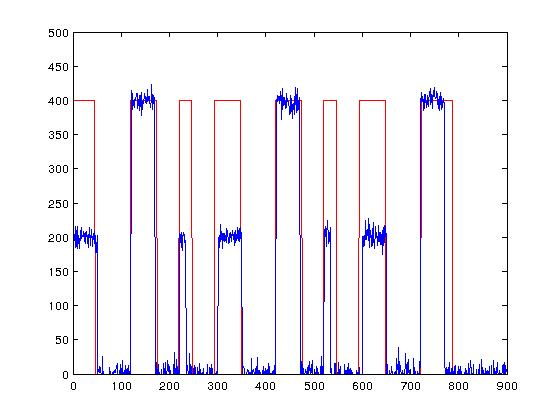
\includegraphics[height = 7.3 cm]{time_freq_model.jpg}
\caption{}
\label{fig:hvb}
\end{figure}

\begin{figure}[h]
\centering
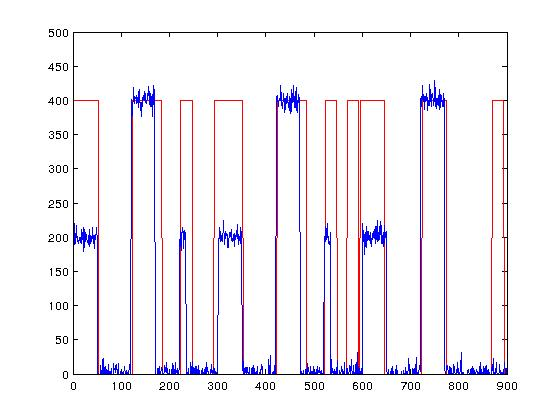
\includegraphics[height = 7.3 cm]{time_freq_1.jpg}
\caption{}
\label{fig:hvb}
\end{figure}

\begin{figure}[h]
\centering
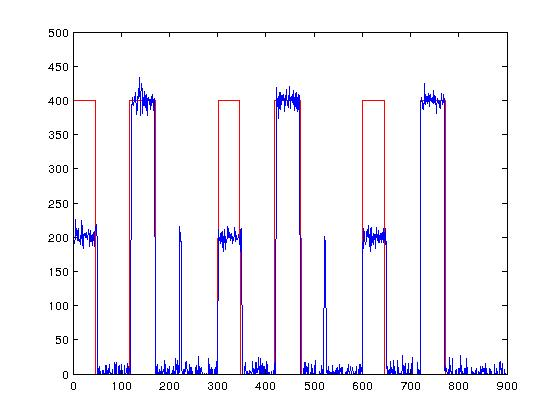
\includegraphics[height = 7.3 cm]{time_freq_missing.jpg}
\caption{}
\label{fig:hvb}
\end{figure}


\bibliography{cswireless2}
\end{document}